\documentclass{standalone}

\usepackage{fontspec}
\setromanfont{Merriweather Regular}
\setsansfont{MerriweatherSans Regular}
\let\familydefault\sfdefault

\usepackage{xcolor}
\definecolor{pepgray}{HTML}{565656}
\usepackage{tikz}

\begin{document}
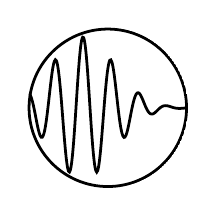
\begin{tikzpicture}
  \begin{scope}
    \clip (0, 0) circle[radius=1cm + 0.5pt];
    \draw[color=black, line width=1pt] (0, 0) circle[radius=1cm];
    \draw[
      color=black,
      line width=1pt,
      smooth,
      scale=0.9,
      xshift=-0.35cm,
      domain=-1.5:3,
      samples=200,
    ] plot (0.63 * \x, {exp(-\x * \x) * cos(10 * deg(\x))}); 
  \end{scope}
\end{tikzpicture}  
\end{document}
